\section{Exploratory data analysis}

\subsection{Purpose of this stage}

The raw-data audit and splitting stages created a corrected interim dataset, a clean modelling table, and a held-out train-test split. This section performs exploratory data analysis using only the training set.

This restriction is methodological. Exploratory findings can influence later modelling choices, including feature engineering, transformations, rule-based baselines, model selection, outlier treatment, and interpretation. Therefore, feature distributions and feature-target relationships are not inspected on the held-out test set.

The goals of this stage are to understand the training data, identify modelling-relevant patterns, and produce report-ready figures and tables while preserving the test set for final evaluation. Large figures are split when needed for readability; a figure is kept in the main text when it is directly used for interpretation, while purely supplementary diagnostics can be moved to an appendix in later stages.

\subsection{Training-set overview}

The dataset used in this section contains 5634 observations. It has 19 feature columns and the binary target column \texttt{Churn\_binary}. No missing values remain after the raw audit and deterministic \texttt{TotalCharges} correction.

\begin{table}[H]
\centering
\caption{Training-set overview}
\begin{tabular}{lr}
\toprule
Item & Value \\
\midrule
Training rows & 5634 \\
Training columns & 20 \\
Missing values & 0 \\
Columns with missing values & 0 \\
Duplicate feature-target rows & 15 \\
\bottomrule
\end{tabular}
\end{table}

The duplicate feature-target rows are not treated as a data-quality issue. The unique customer identifier was intentionally removed before modelling, so different customers can legitimately share the same observed feature values and churn label.

\subsection{Target distribution}

The positive class is churn, encoded as \texttt{1}. The target distribution remains moderately imbalanced, with churn representing 26.54\% of observations.

\begin{table}[H]
\centering
\caption{Target distribution}
\begin{tabular}{lrr}
\toprule
\texttt{Churn\_binary} & Count & Percentage \\
\midrule
0 & 4139 & 73.46 \\
1 & 1495 & 26.54 \\
\bottomrule
\end{tabular}
\end{table}

This imbalance is not extreme, but it is large enough that accuracy alone will be an incomplete evaluation metric. Later modelling sections should include metrics that distinguish false positives from false negatives, such as precision, recall, specificity, F1-score, ROC-AUC, PR-AUC, and threshold analysis.

\subsection{Numeric feature summary}

The dataset has three numeric features: \texttt{tenure}, \texttt{MonthlyCharges}, and \texttt{TotalCharges}. Numeric summaries are computed on this development split only.

\begin{table}[H]
\centering
\caption{Numeric feature summary}
\begin{tabular}{lrrrrrrrr}
\toprule
Feature & Count & Mean & Std. & Min & 25\% & Median & 75\% & Max \\
\midrule
\texttt{tenure} & 5634 & 32.49 & 24.57 & 0.00 & 9.00 & 29.00 & 55.00 & 72.00 \\
\texttt{MonthlyCharges} & 5634 & 64.93 & 30.14 & 18.40 & 35.66 & 70.50 & 90.00 & 118.75 \\
\texttt{TotalCharges} & 5634 & 2299.33 & 2279.20 & 0.00 & 402.98 & 1394.93 & 3835.83 & 8684.80 \\
\bottomrule
\end{tabular}
\end{table}

The numeric variables have different scales. This matters for later model families such as k-nearest neighbours, support vector machines, logistic regression with regularization, and neural networks, where scaling is usually required. Scaling should be fitted inside training-only pipelines rather than on the full dataset.

\subsection{Numeric feature distributions}

Figure \ref{fig:training-numeric-distributions} shows histograms and boxplots for the three numeric features in this split.

\begin{figure}[H]
\centering
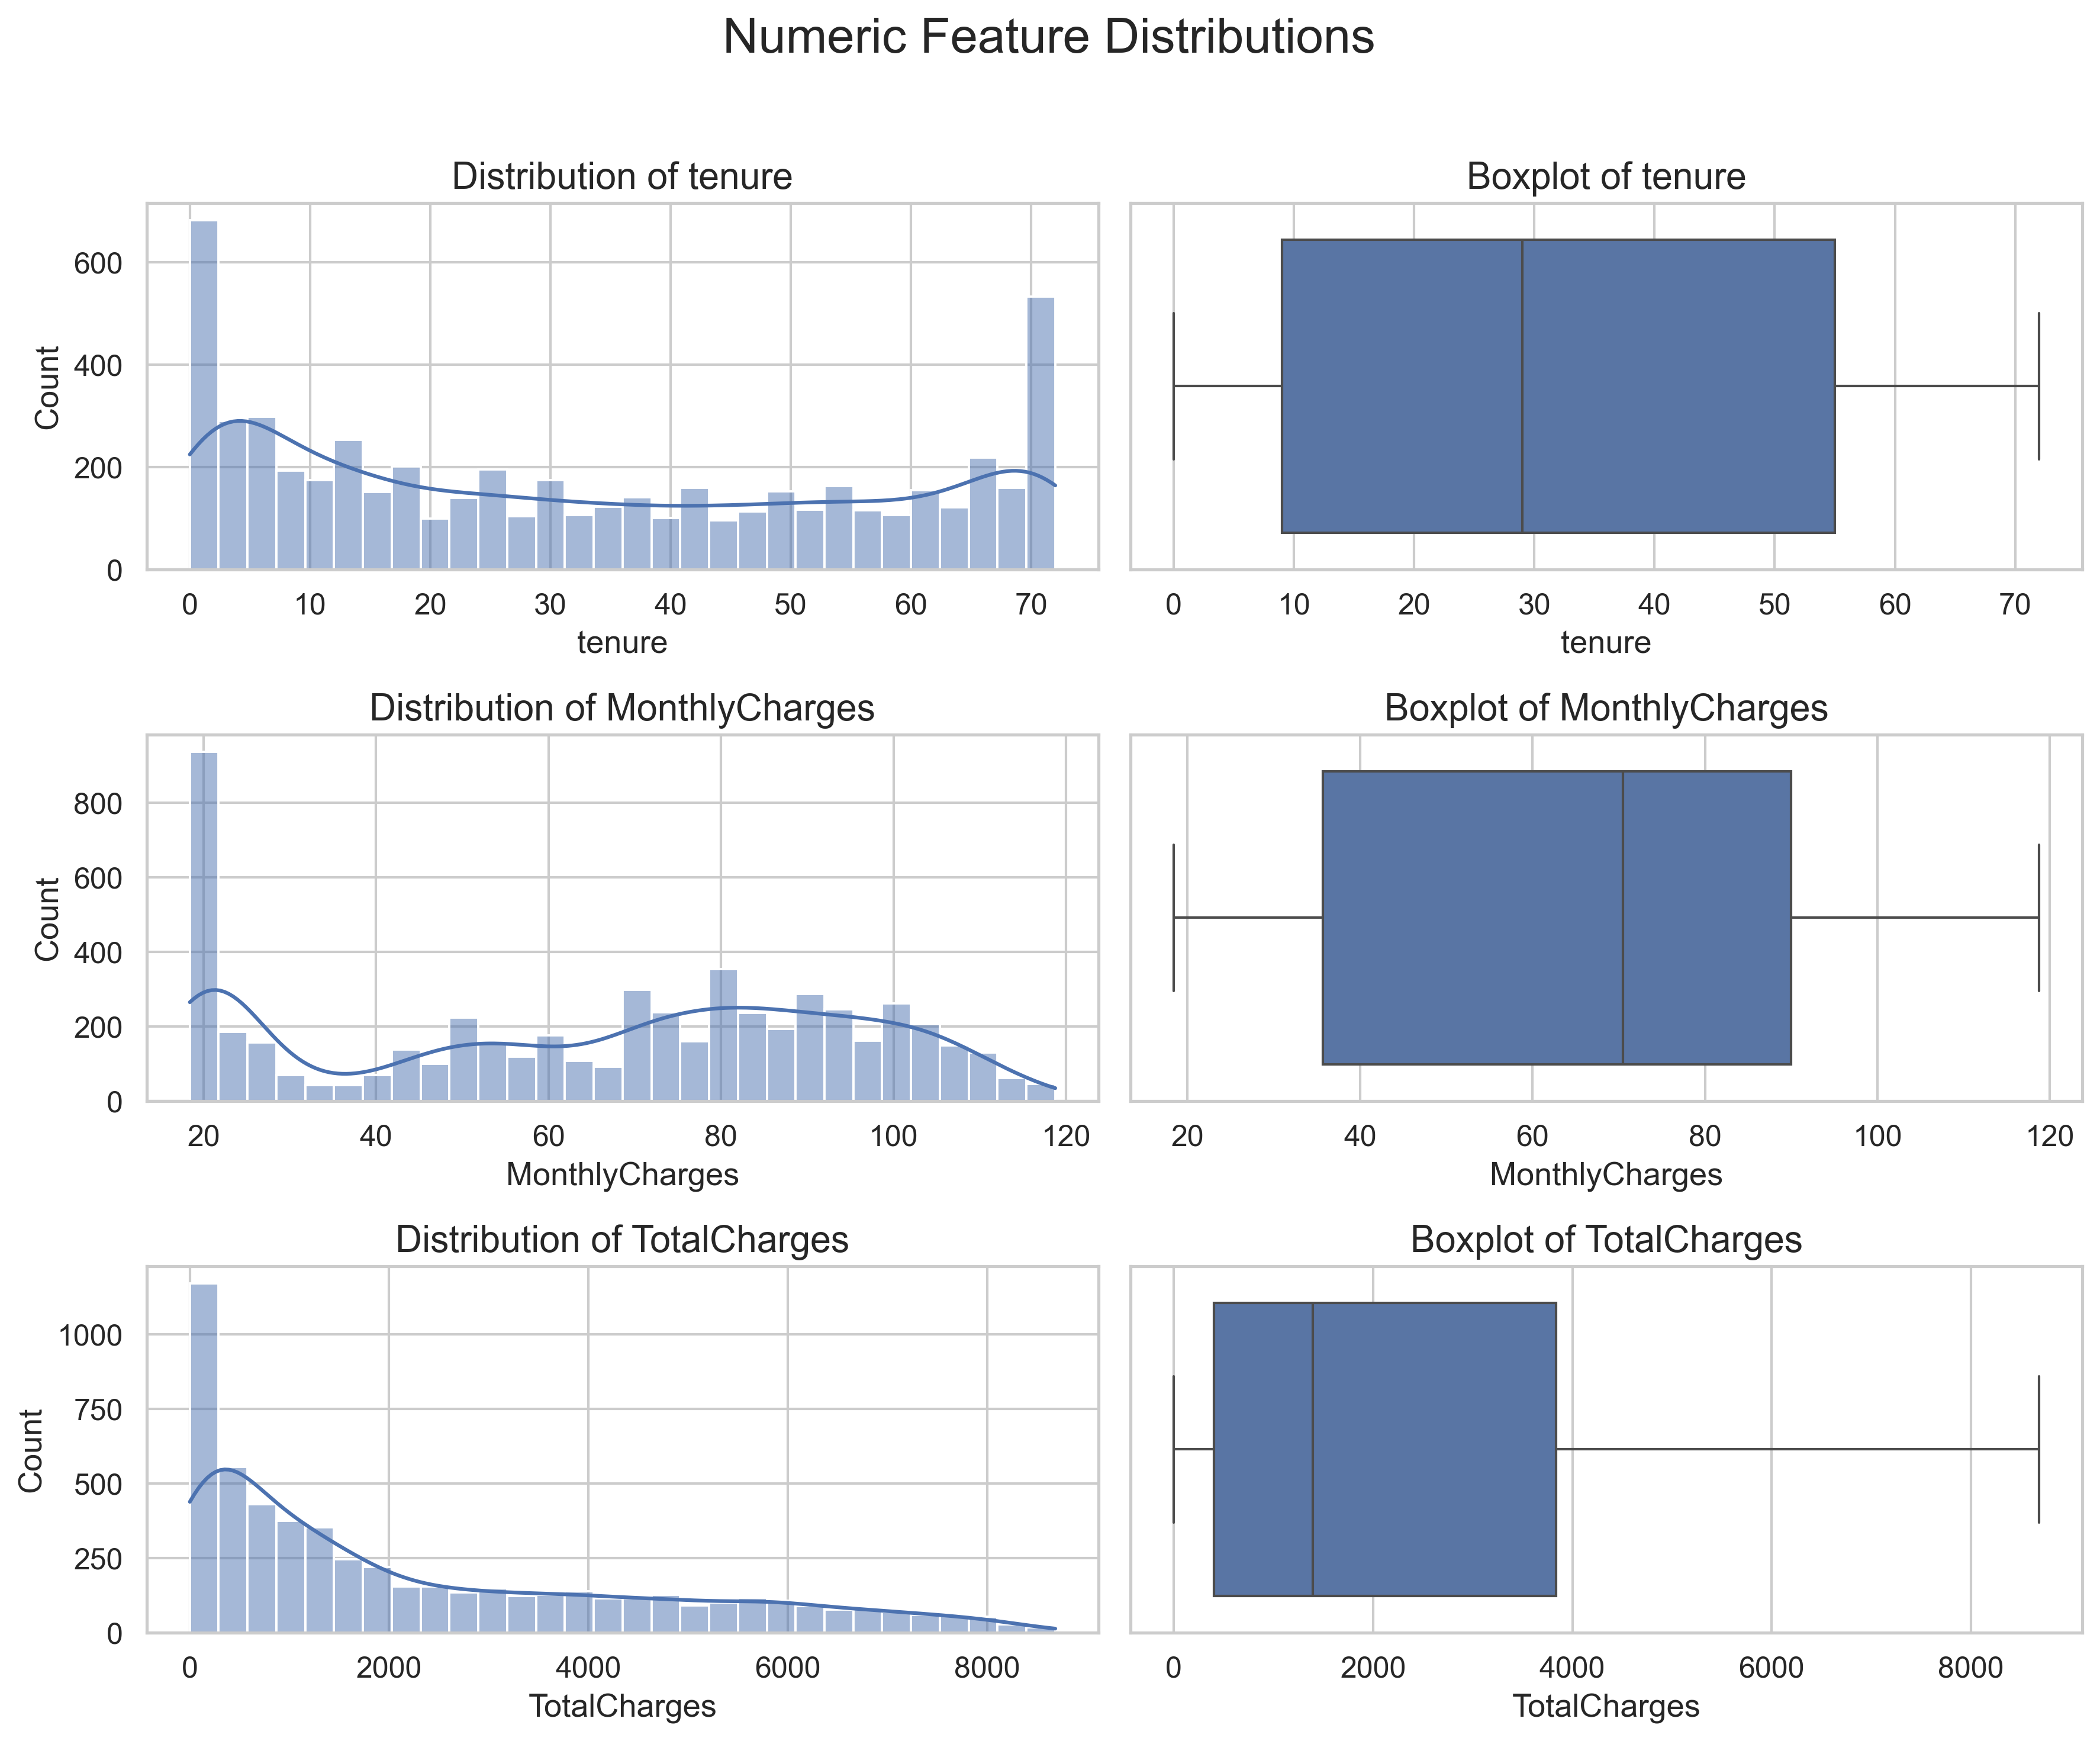
\includegraphics[width=\textwidth]{../figures/training_numeric_feature_distributions.png}
\caption{Numeric feature distributions and boxplots}
\label{fig:training-numeric-distributions}
\end{figure}

The distribution of \texttt{tenure} has substantial mass near low values and also many observations near the upper end of the observed range. This indicates that the training set contains both newly joined customers and long-tenure customers.

The distribution of \texttt{MonthlyCharges} is not symmetric. There is a large group of customers with relatively low monthly charges and a broad group at higher monthly charge levels. The distribution of \texttt{TotalCharges} is strongly right-skewed. This is expected because total charges accumulate over time: many customers have low accumulated charges, while long-tenure or high-monthly-charge customers can have much larger accumulated totals.

These plots are descriptive. They do not justify automatic outlier removal. The raw audit already checked for impossible negative numeric values. High but plausible values should be treated as potential natural observations unless there is separate evidence that they are coding errors.

\subsection{Numeric feature distributions by churn}

Figure \ref{fig:training-numeric-by-churn} compares the numeric feature distributions between churners and non-churners.

\begin{figure}[H]
\centering
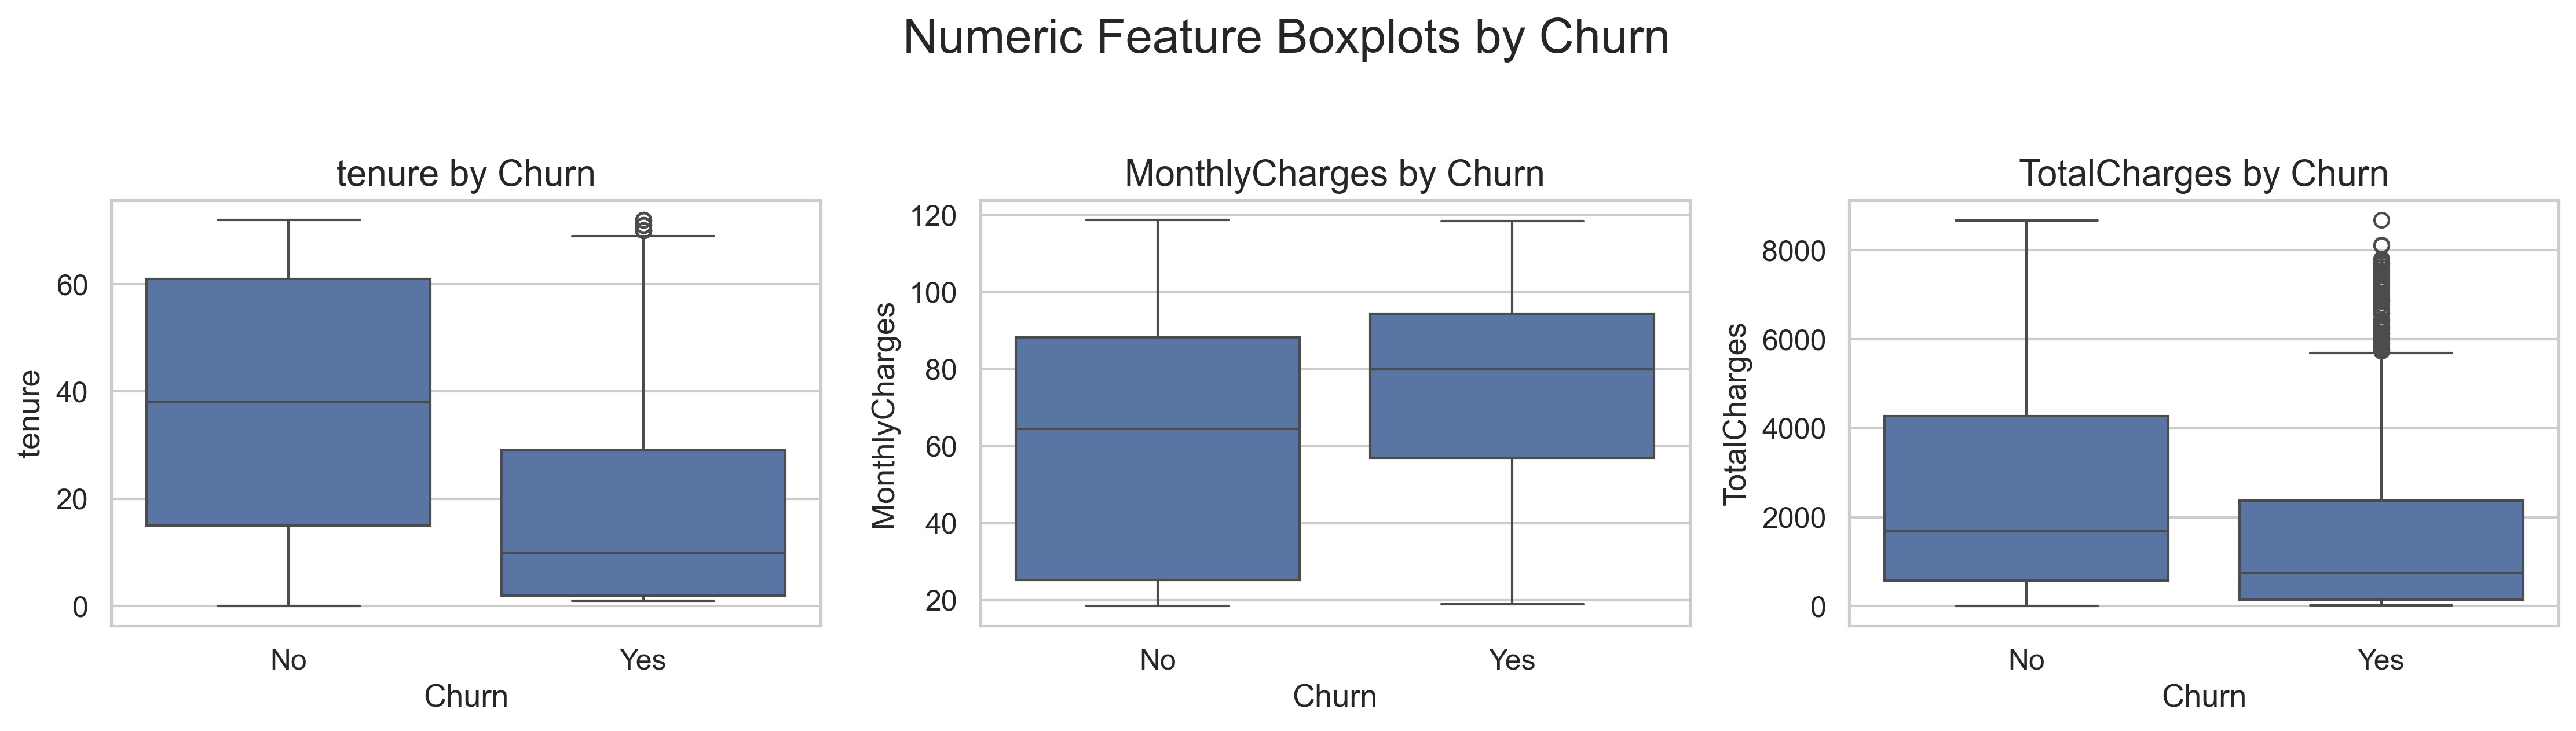
\includegraphics[width=\textwidth]{../figures/training_numeric_feature_boxplots_by_churn.png}
\caption{Numeric feature boxplots by churn}
\label{fig:training-numeric-by-churn}
\end{figure}

The class-conditioned boxplots show clearer feature-target structure than the marginal distributions. Customers who churned have substantially lower \texttt{tenure} than customers who did not churn. This is one of the strongest numeric patterns in the training data and suggests that newer customers are more likely to leave.

\texttt{MonthlyCharges} tends to be higher for churners. This indicates that customers with higher monthly bills may be at greater churn risk, at least as a marginal training-set association. \texttt{TotalCharges} tends to be lower for churners, but this should be interpreted carefully. Since \texttt{TotalCharges} accumulates over time, lower total charges among churners are consistent with churners having shorter tenure.

\subsection{Numeric scatter matrix}

Figure \ref{fig:training-scatter-matrix} shows a scatter matrix for the numeric features, coloured by churn status.

\begin{figure}[H]
\centering
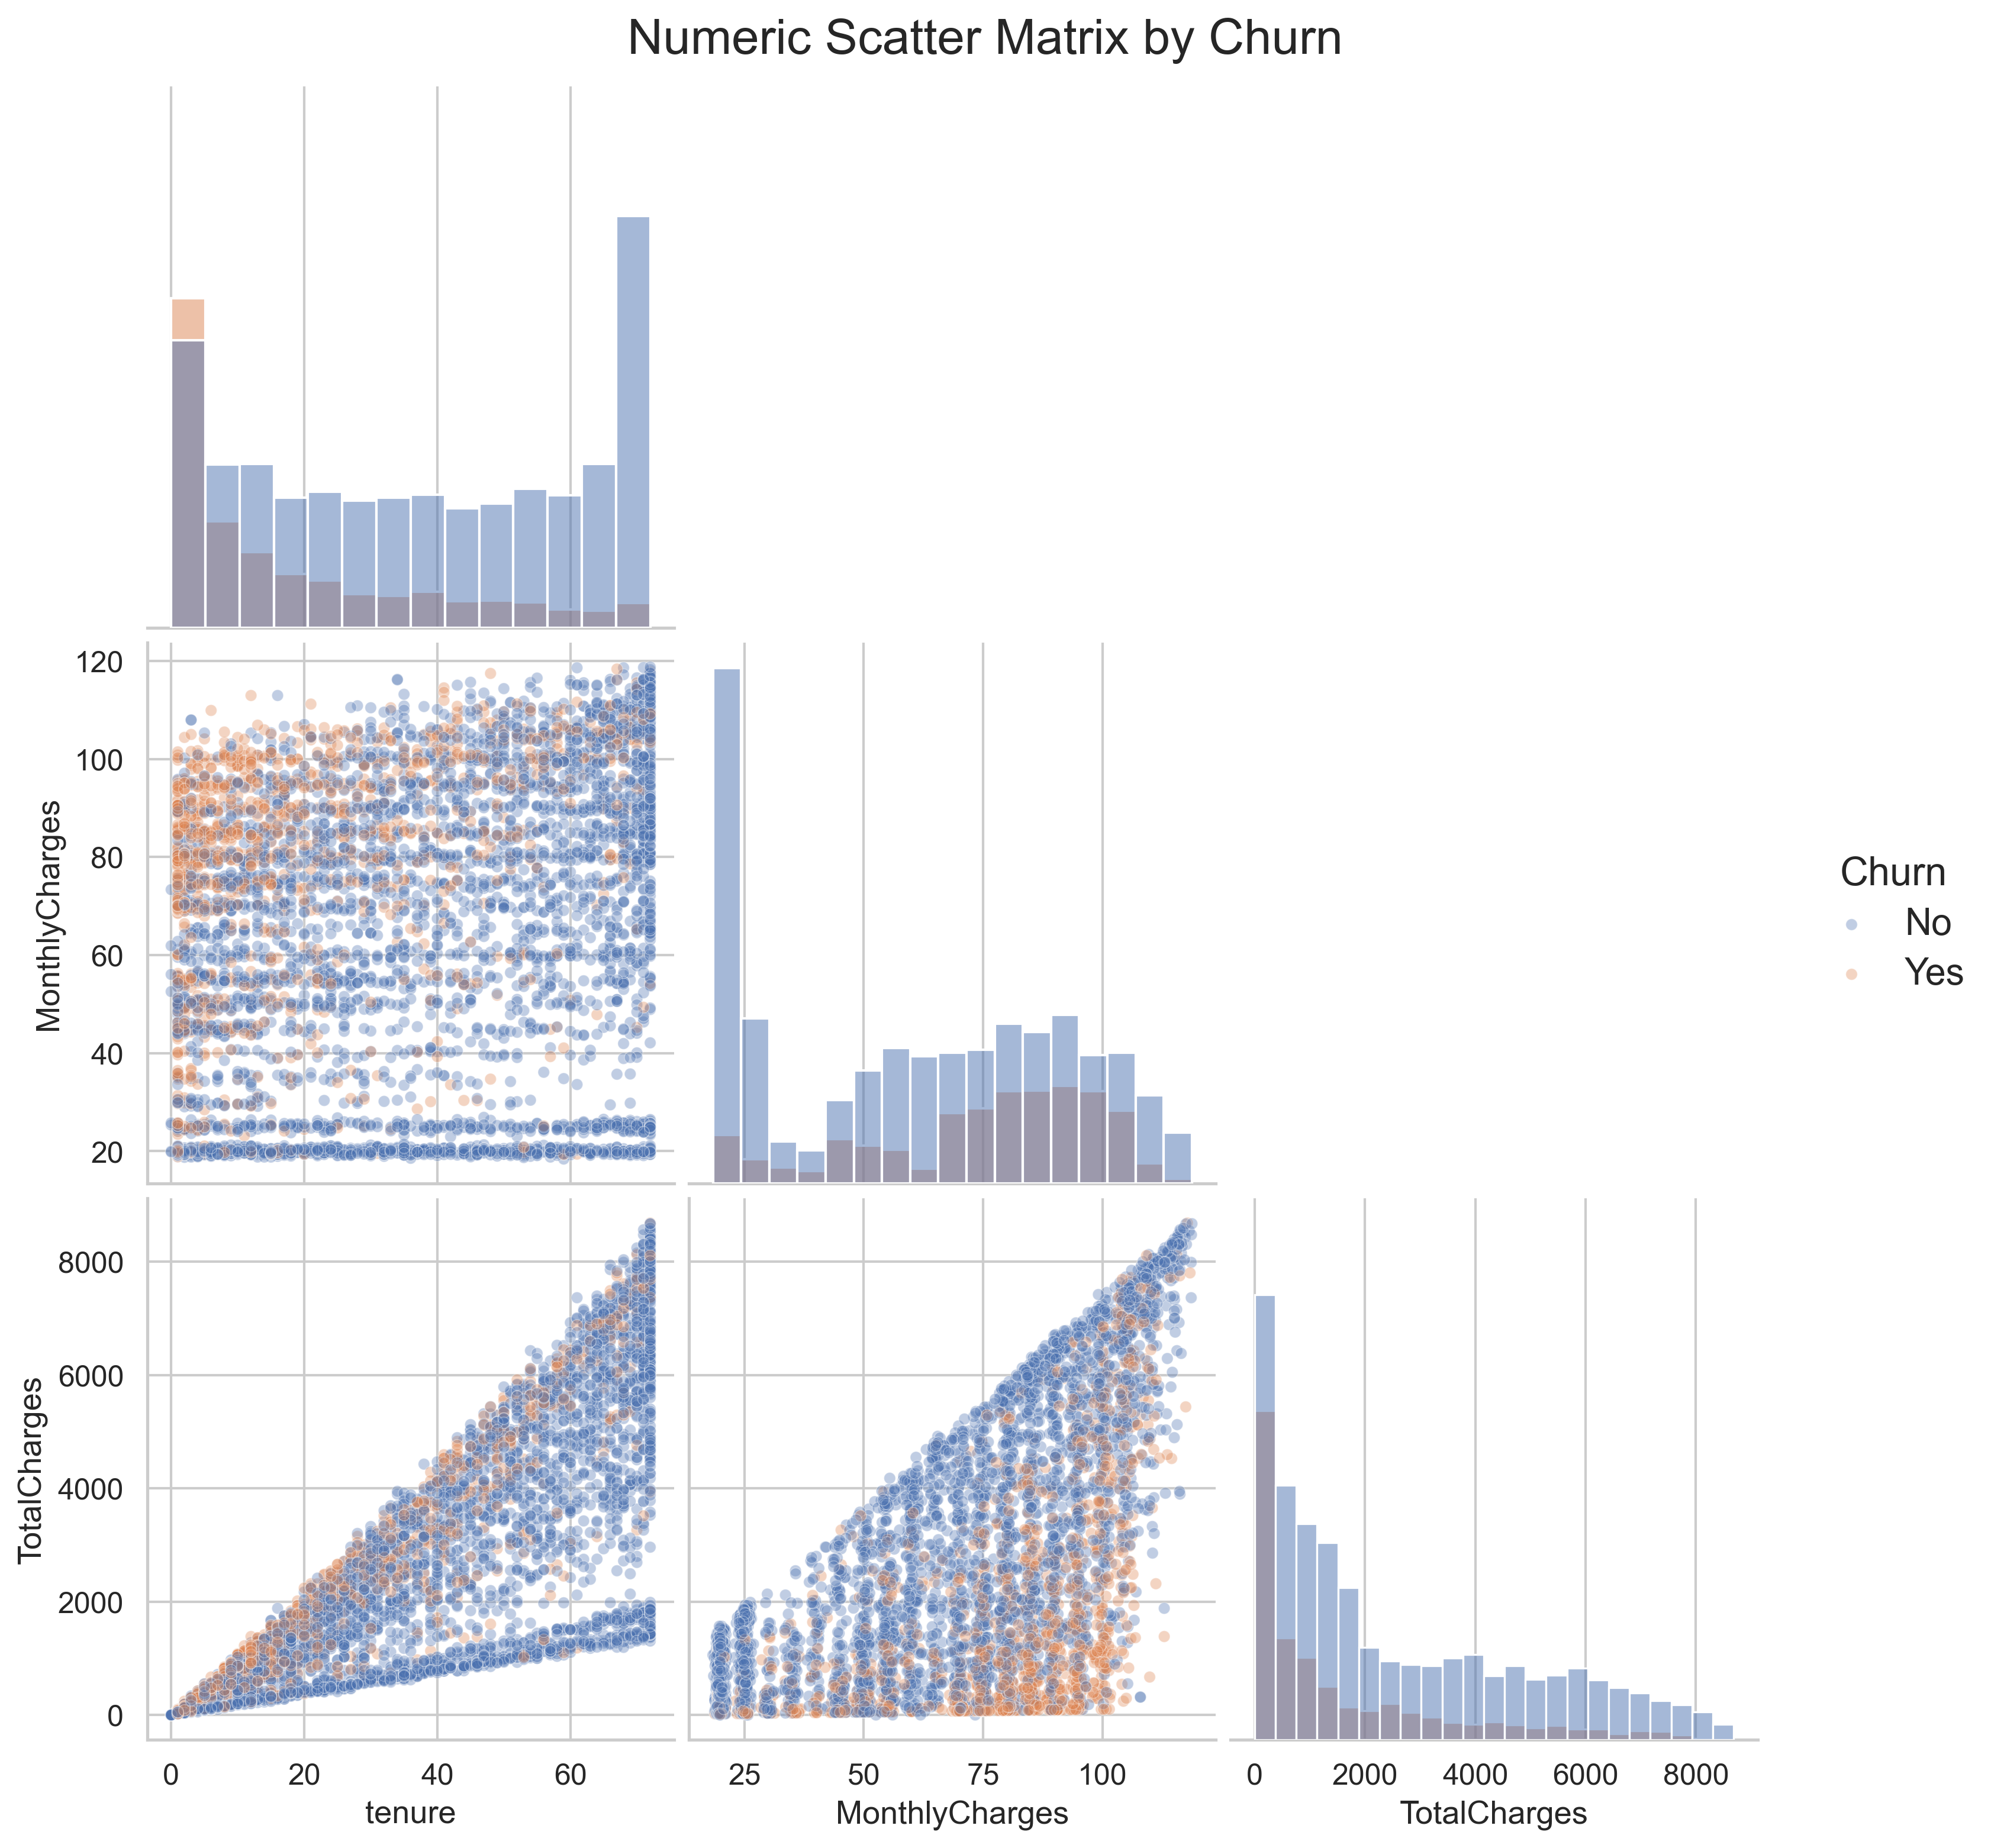
\includegraphics[width=0.88\textwidth]{../figures/training_numeric_scatter_matrix_by_churn.png}
\caption{Numeric scatter matrix by churn}
\label{fig:training-scatter-matrix}
\end{figure}

The scatter matrix shows visible churn-related patterns, but it does not show a clean visual separation between churners and non-churners using any single pair of numeric variables. Churners are more concentrated among customers with shorter tenure and are also relatively visible among customers with higher monthly charges. However, the two classes overlap substantially across the numeric feature space, suggesting that churn is not separable by a simple pairwise numeric boundary.

The clearest structural pattern is the relationship between \texttt{tenure} and \texttt{TotalCharges}. The triangular shape is expected because total charges accumulate over months and are also affected by monthly charges. For a fixed tenure, customers with higher monthly charges can accumulate higher total charges. This motivates using models that can combine numeric and categorical information, and possibly models that can learn interactions.

\subsection{Numeric correlation matrix}

Figure \ref{fig:training-numeric-correlation} shows the Pearson correlation matrix among numeric features and \texttt{Churn\_binary} in this split.

\begin{figure}[H]
\centering
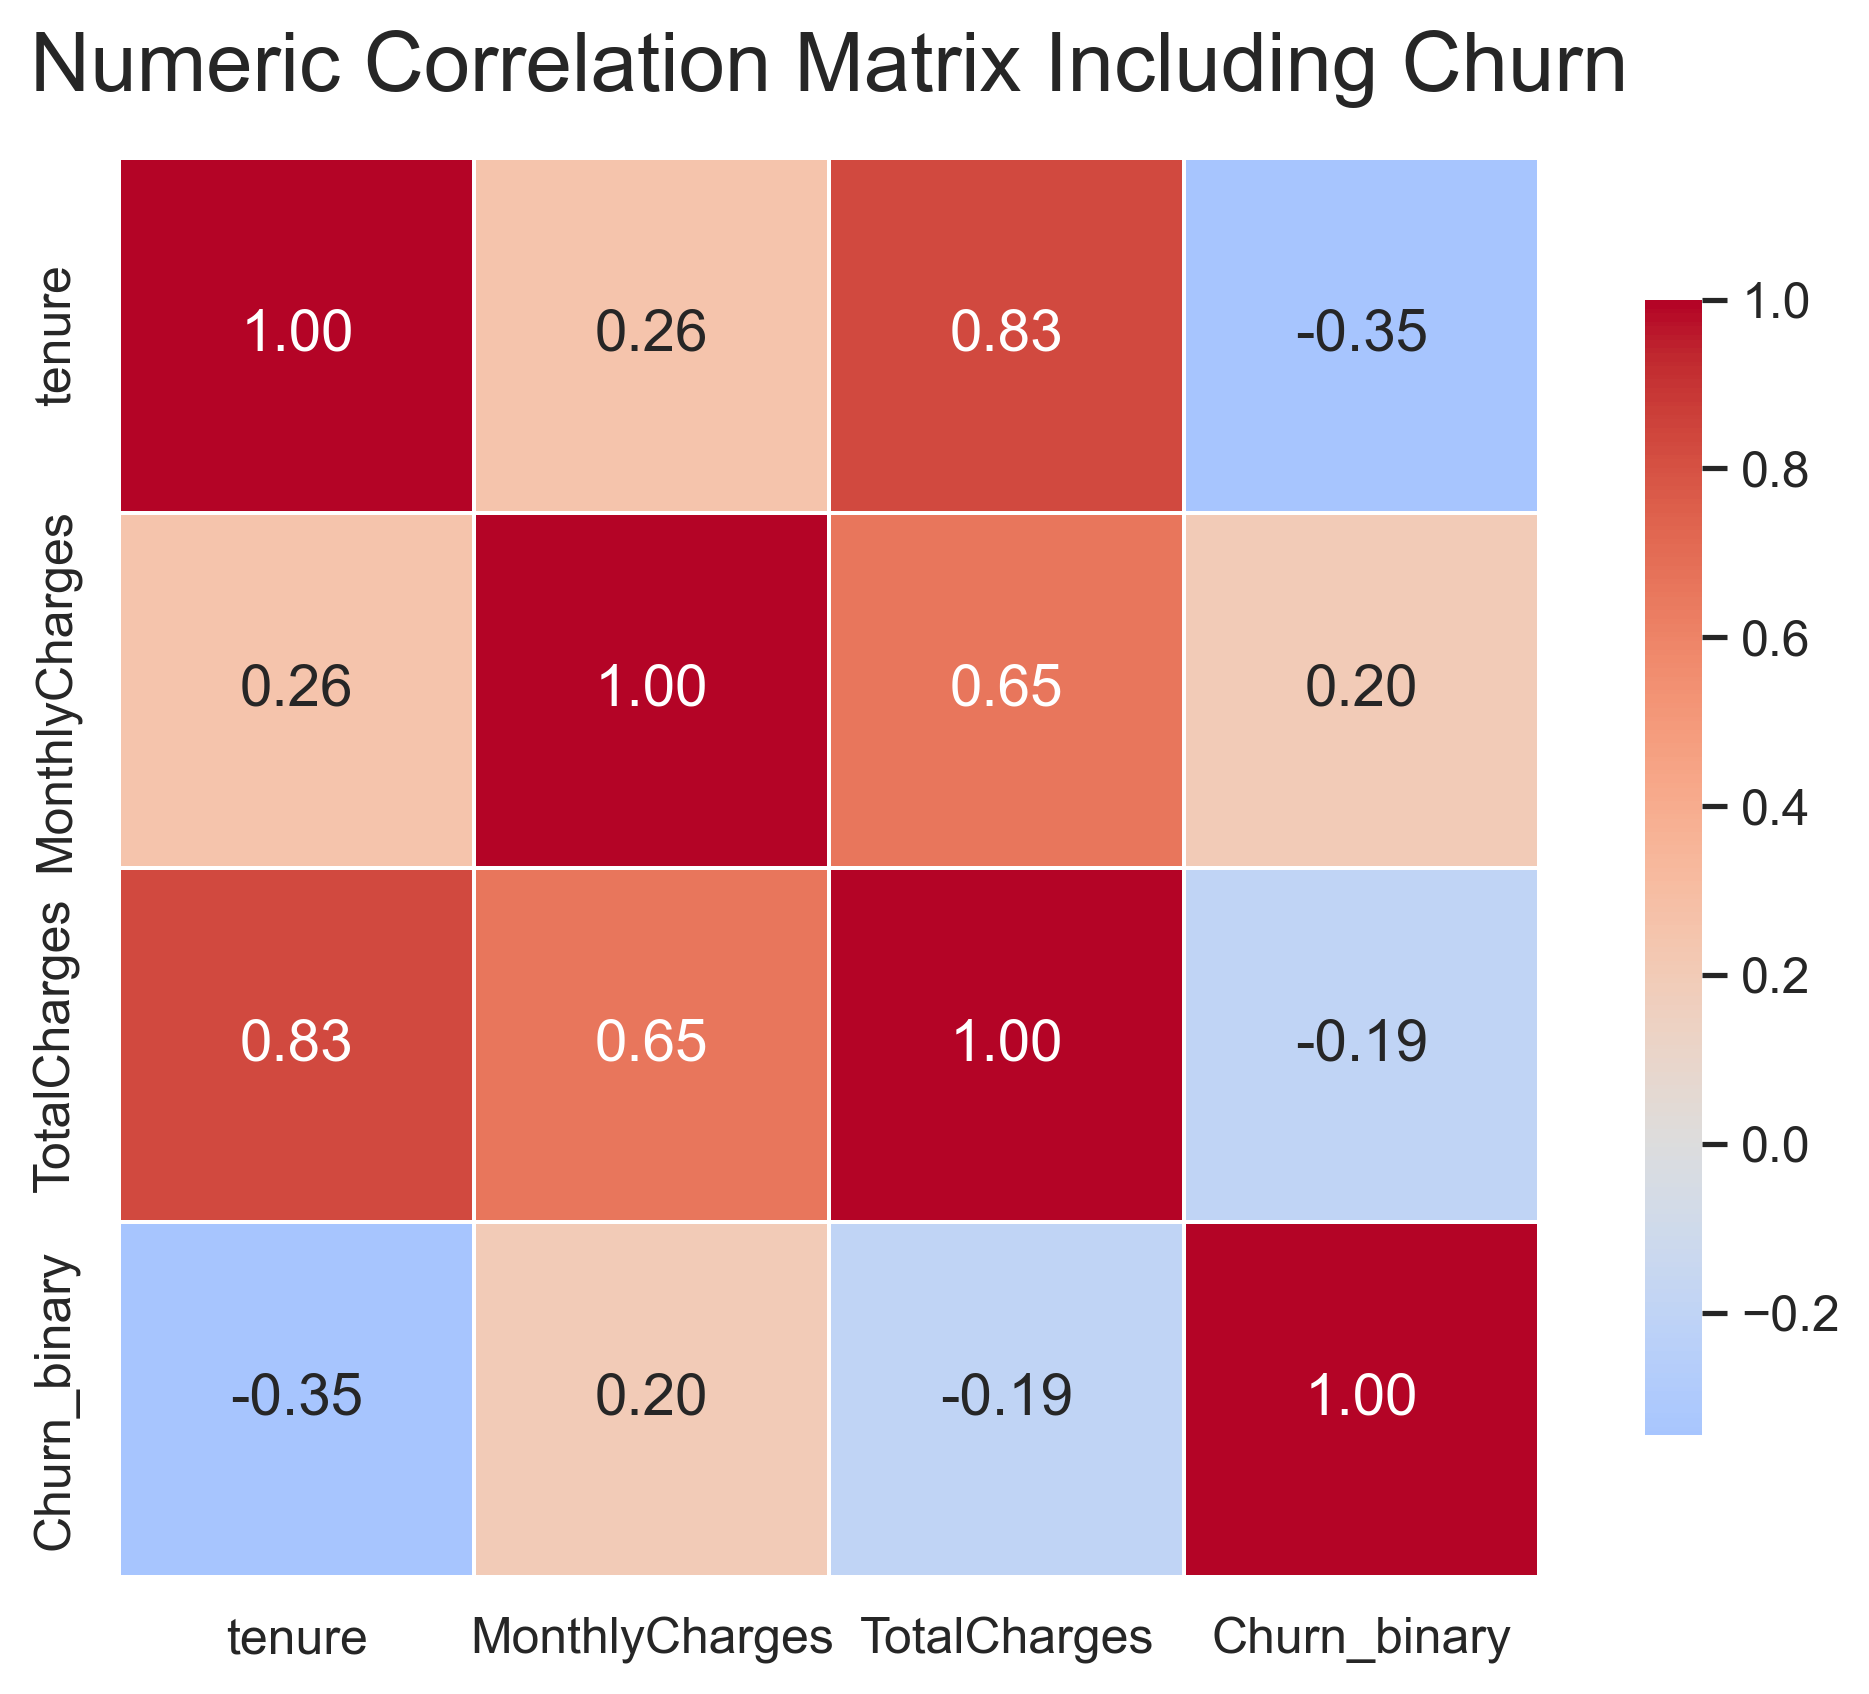
\includegraphics[width=0.55\textwidth]{../figures/training_numeric_correlation_matrix.png}
\caption{Numeric correlation matrix including \texttt{Churn\_binary}}
\label{fig:training-numeric-correlation}
\end{figure}

The strongest numeric correlation with churn is for \texttt{tenure}, with correlation approximately \(-0.35\). Longer-tenure customers are less likely to churn in the training data. \texttt{MonthlyCharges} has a positive correlation with churn of approximately \(0.20\), while \texttt{TotalCharges} has a negative correlation with churn of approximately \(-0.19\).

The correlation matrix also shows that \texttt{tenure} and \texttt{TotalCharges} are strongly correlated, approximately \(0.83\), and that \texttt{MonthlyCharges} and \texttt{TotalCharges} are also positively correlated, approximately \(0.65\). These are marginal linear associations only. They do not capture nonlinear relationships, interactions, or the effects of categorical variables.

\subsection{Categorical feature frequencies}

Figures \ref{fig:training-categorical-frequencies-part-1} and \ref{fig:training-categorical-frequencies-part-2} show the distribution of categorical feature levels. The categorical variables are split across two figures to keep axis labels and category names readable in the compiled report.

\begin{figure}[H]
\centering
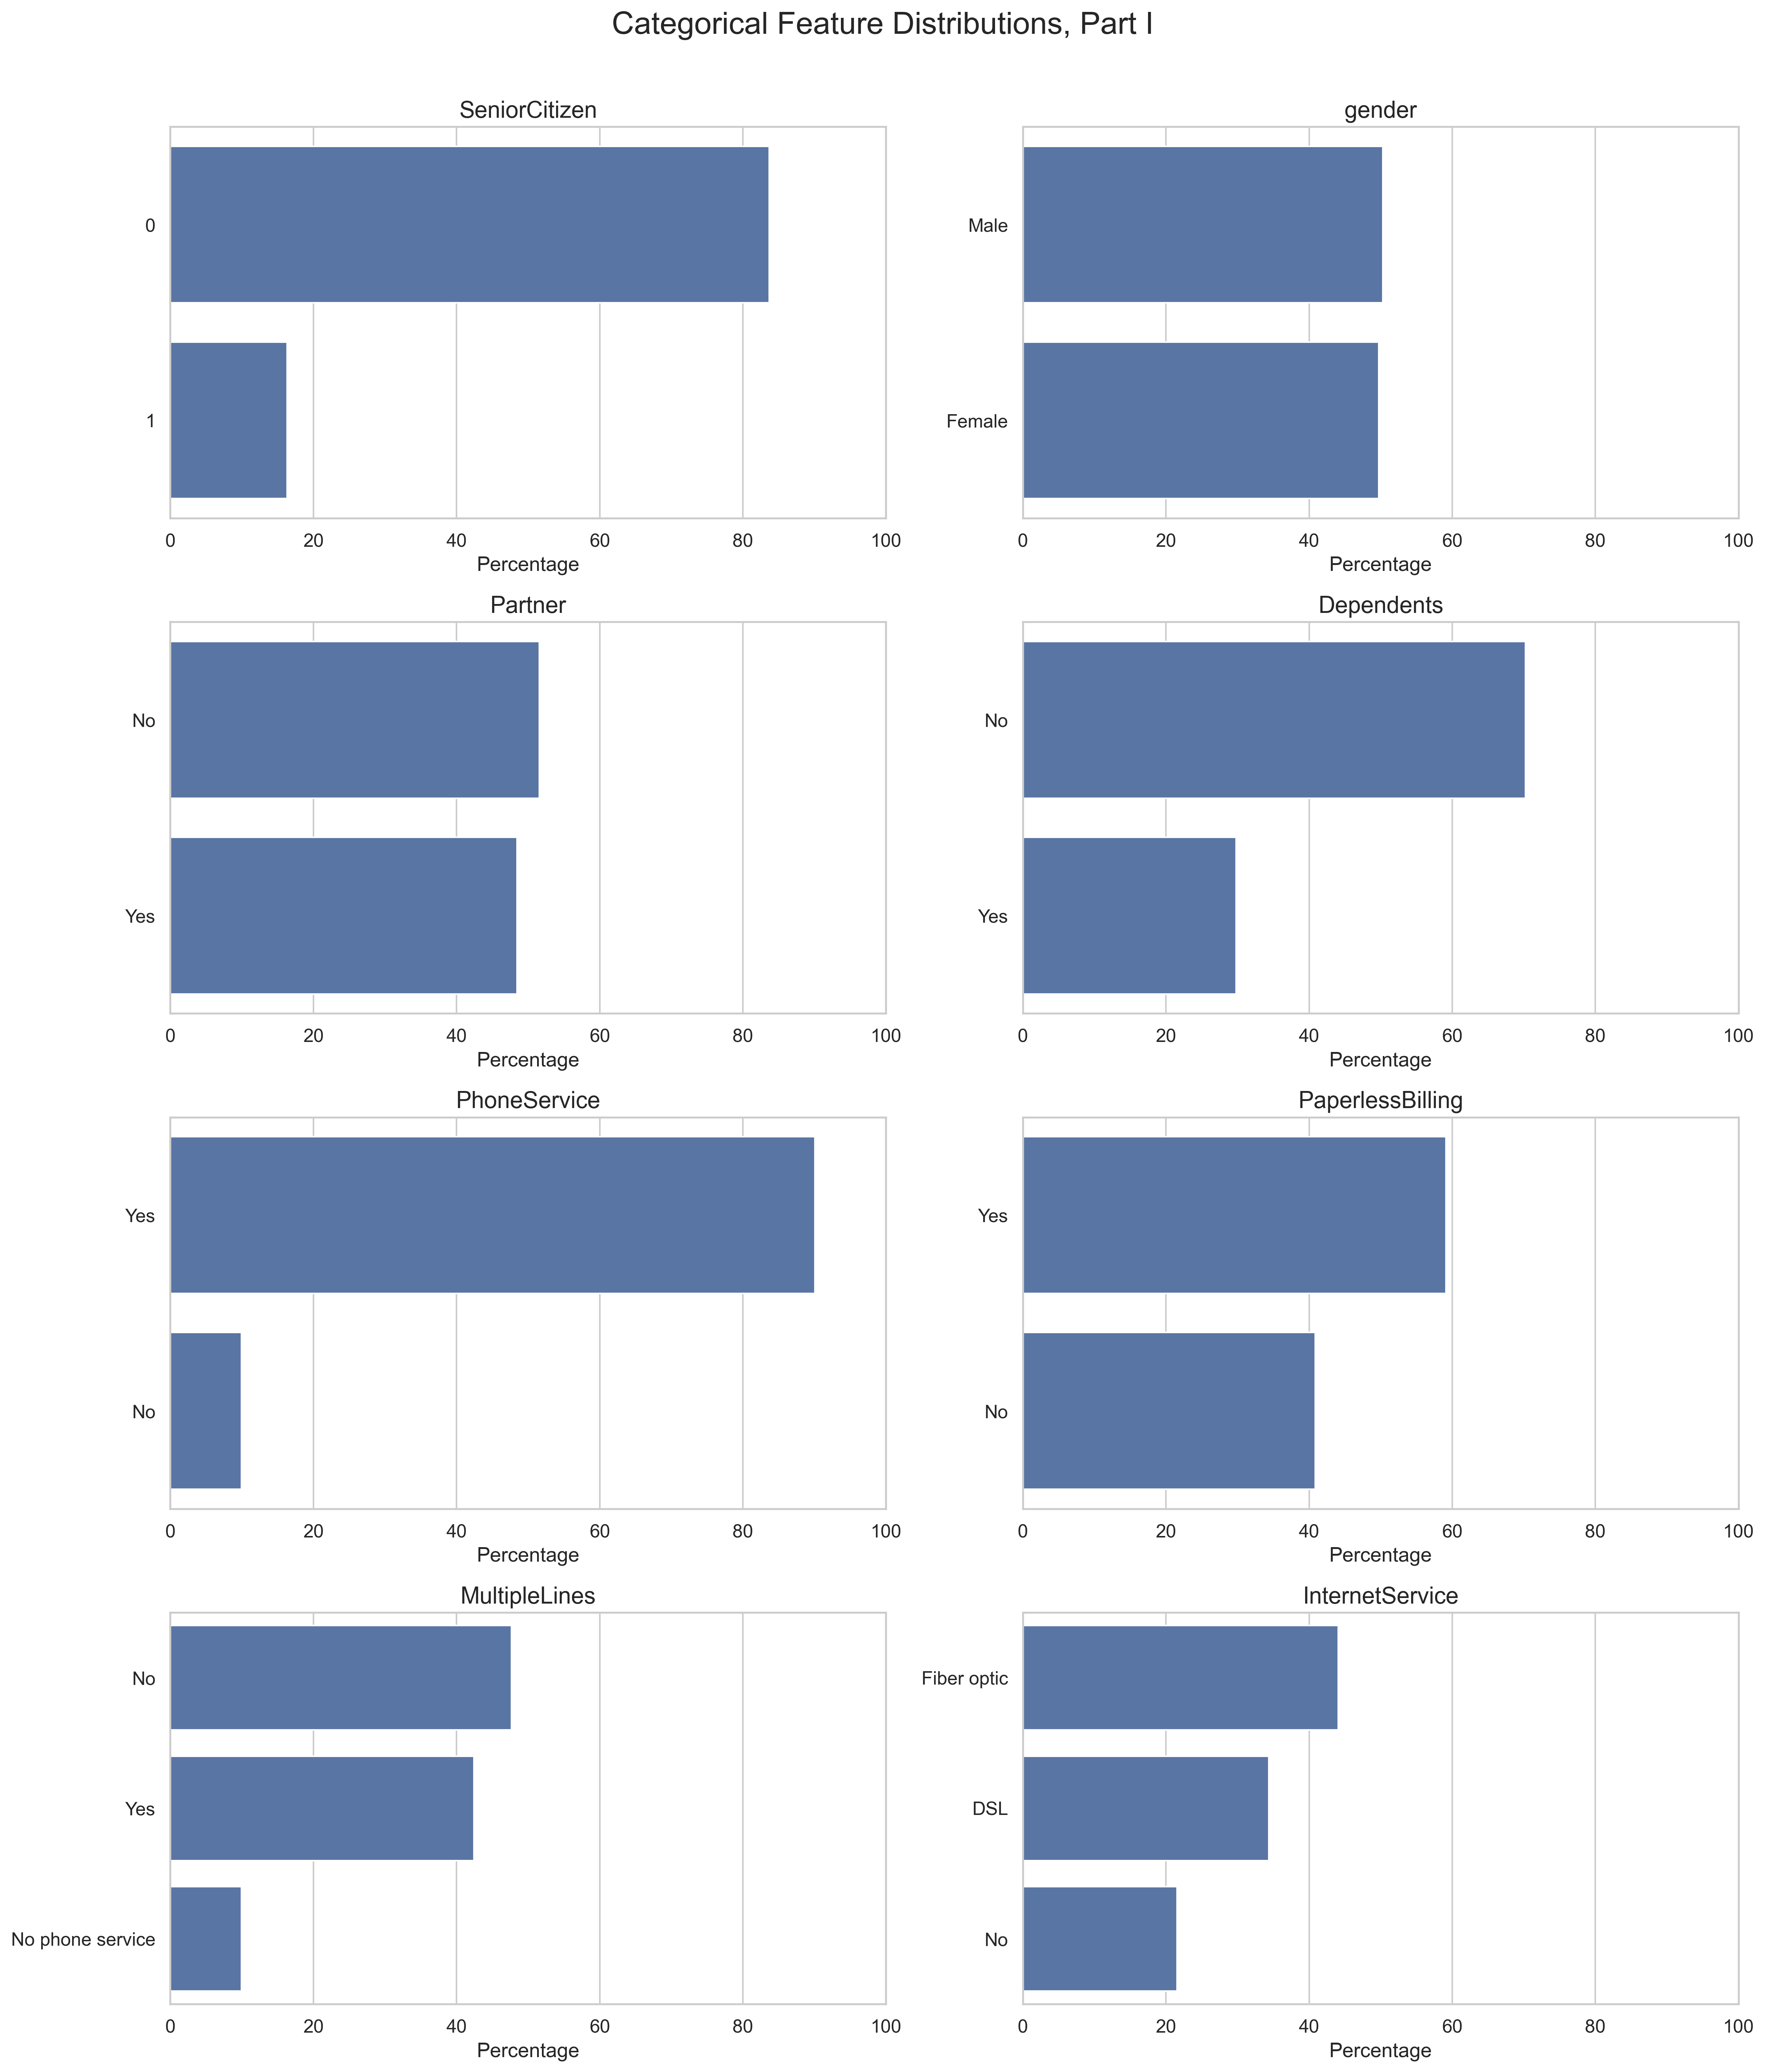
\includegraphics[width=\textwidth]{../figures/training_categorical_feature_frequencies_part_1.png}
\caption{Categorical feature distributions, Part I}
\label{fig:training-categorical-frequencies-part-1}
\end{figure}

\begin{figure}[H]
\centering
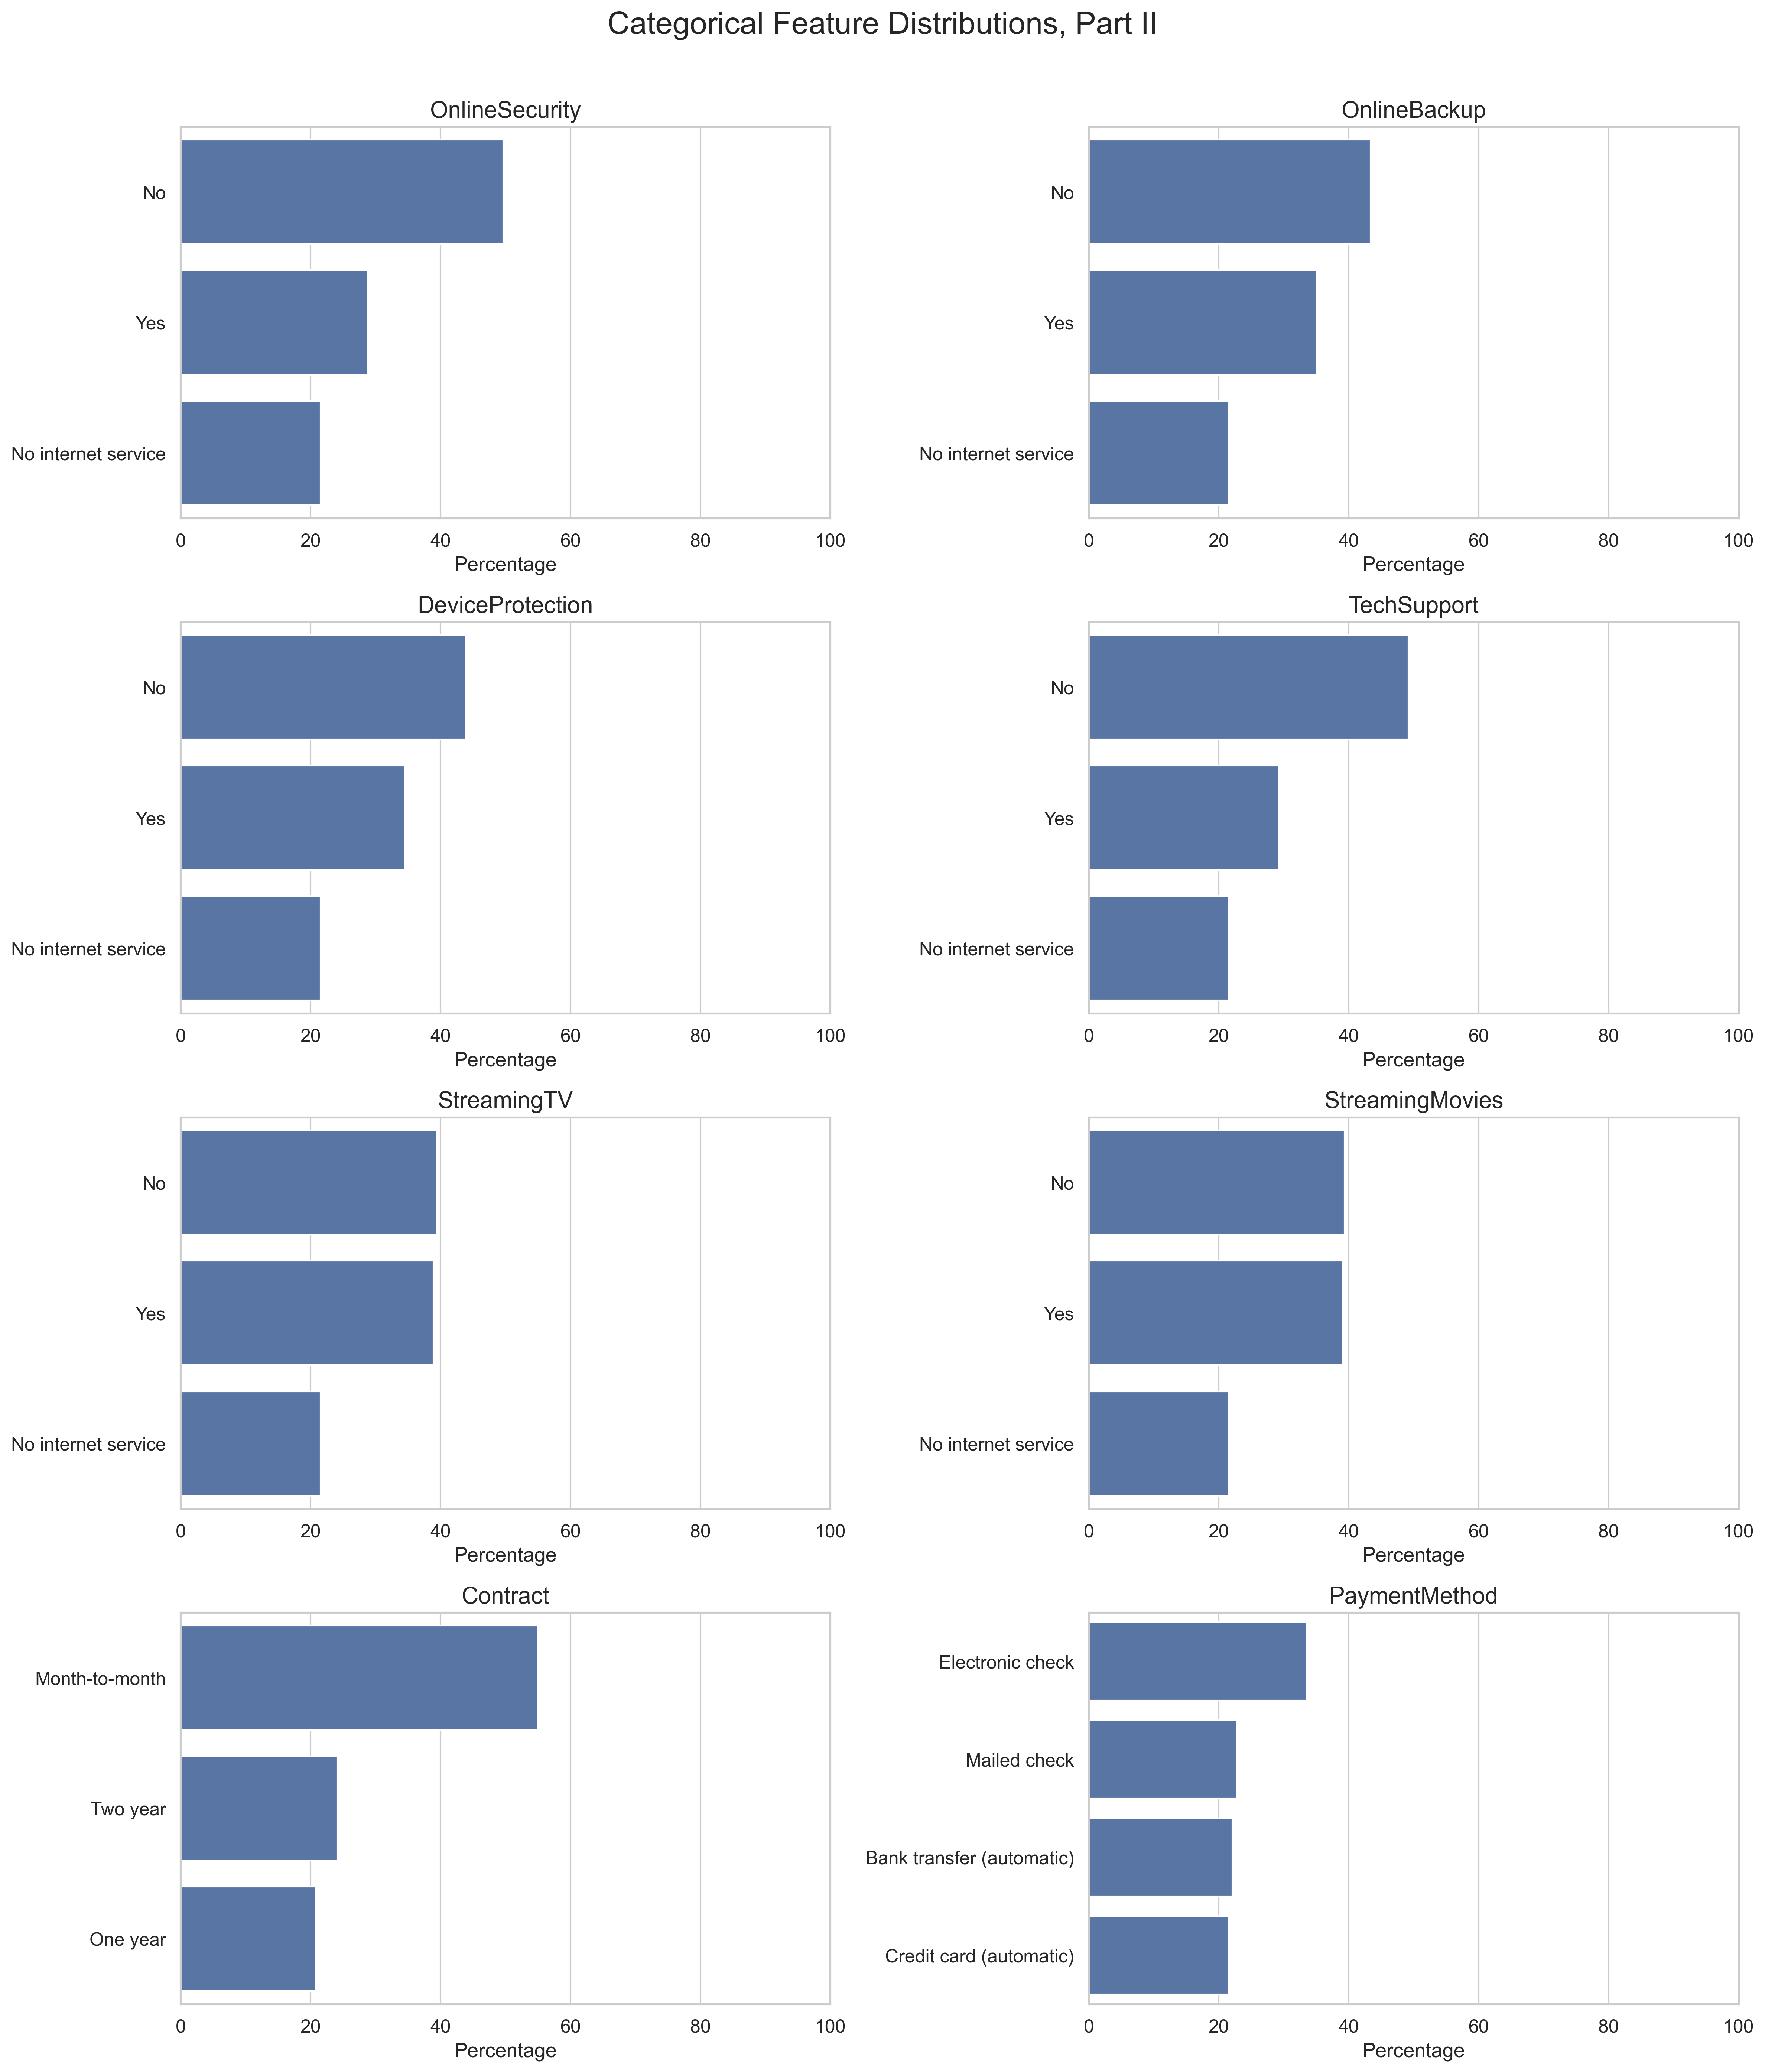
\includegraphics[width=\textwidth]{../figures/training_categorical_feature_frequencies_part_2.png}
\caption{Categorical feature distributions, Part II}
\label{fig:training-categorical-frequencies-part-2}
\end{figure}

Several categorical predictors contain strongly imbalanced levels. For example, \texttt{PhoneService = Yes} represents 90.08\% of the training set, \texttt{SeniorCitizen = 0} represents 83.67\%, and \texttt{Contract = Month-to-month} represents 55.06\%. These imbalances matter because rare levels can create unstable estimates in simple baselines and can affect how much information a model can learn from a category.

Several internet-service add-on variables contain the structural level \texttt{No internet service}. This is not missingness. It is an informative category indicating that the customer does not have internet service. Later preprocessing should preserve this category rather than treating it as a missing value.

\subsection{Categorical churn rates}

Figures \ref{fig:training-categorical-churn-rates-part-1} and \ref{fig:training-categorical-churn-rates-part-2} show the churn rate within each categorical level. Both parts are included in the main section because they support the interpretation: Part I contains demographic, household, billing, phone-service, and internet-service variables, while Part II contains several service add-ons as well as contract type and payment method.

\begin{figure}[H]
\centering
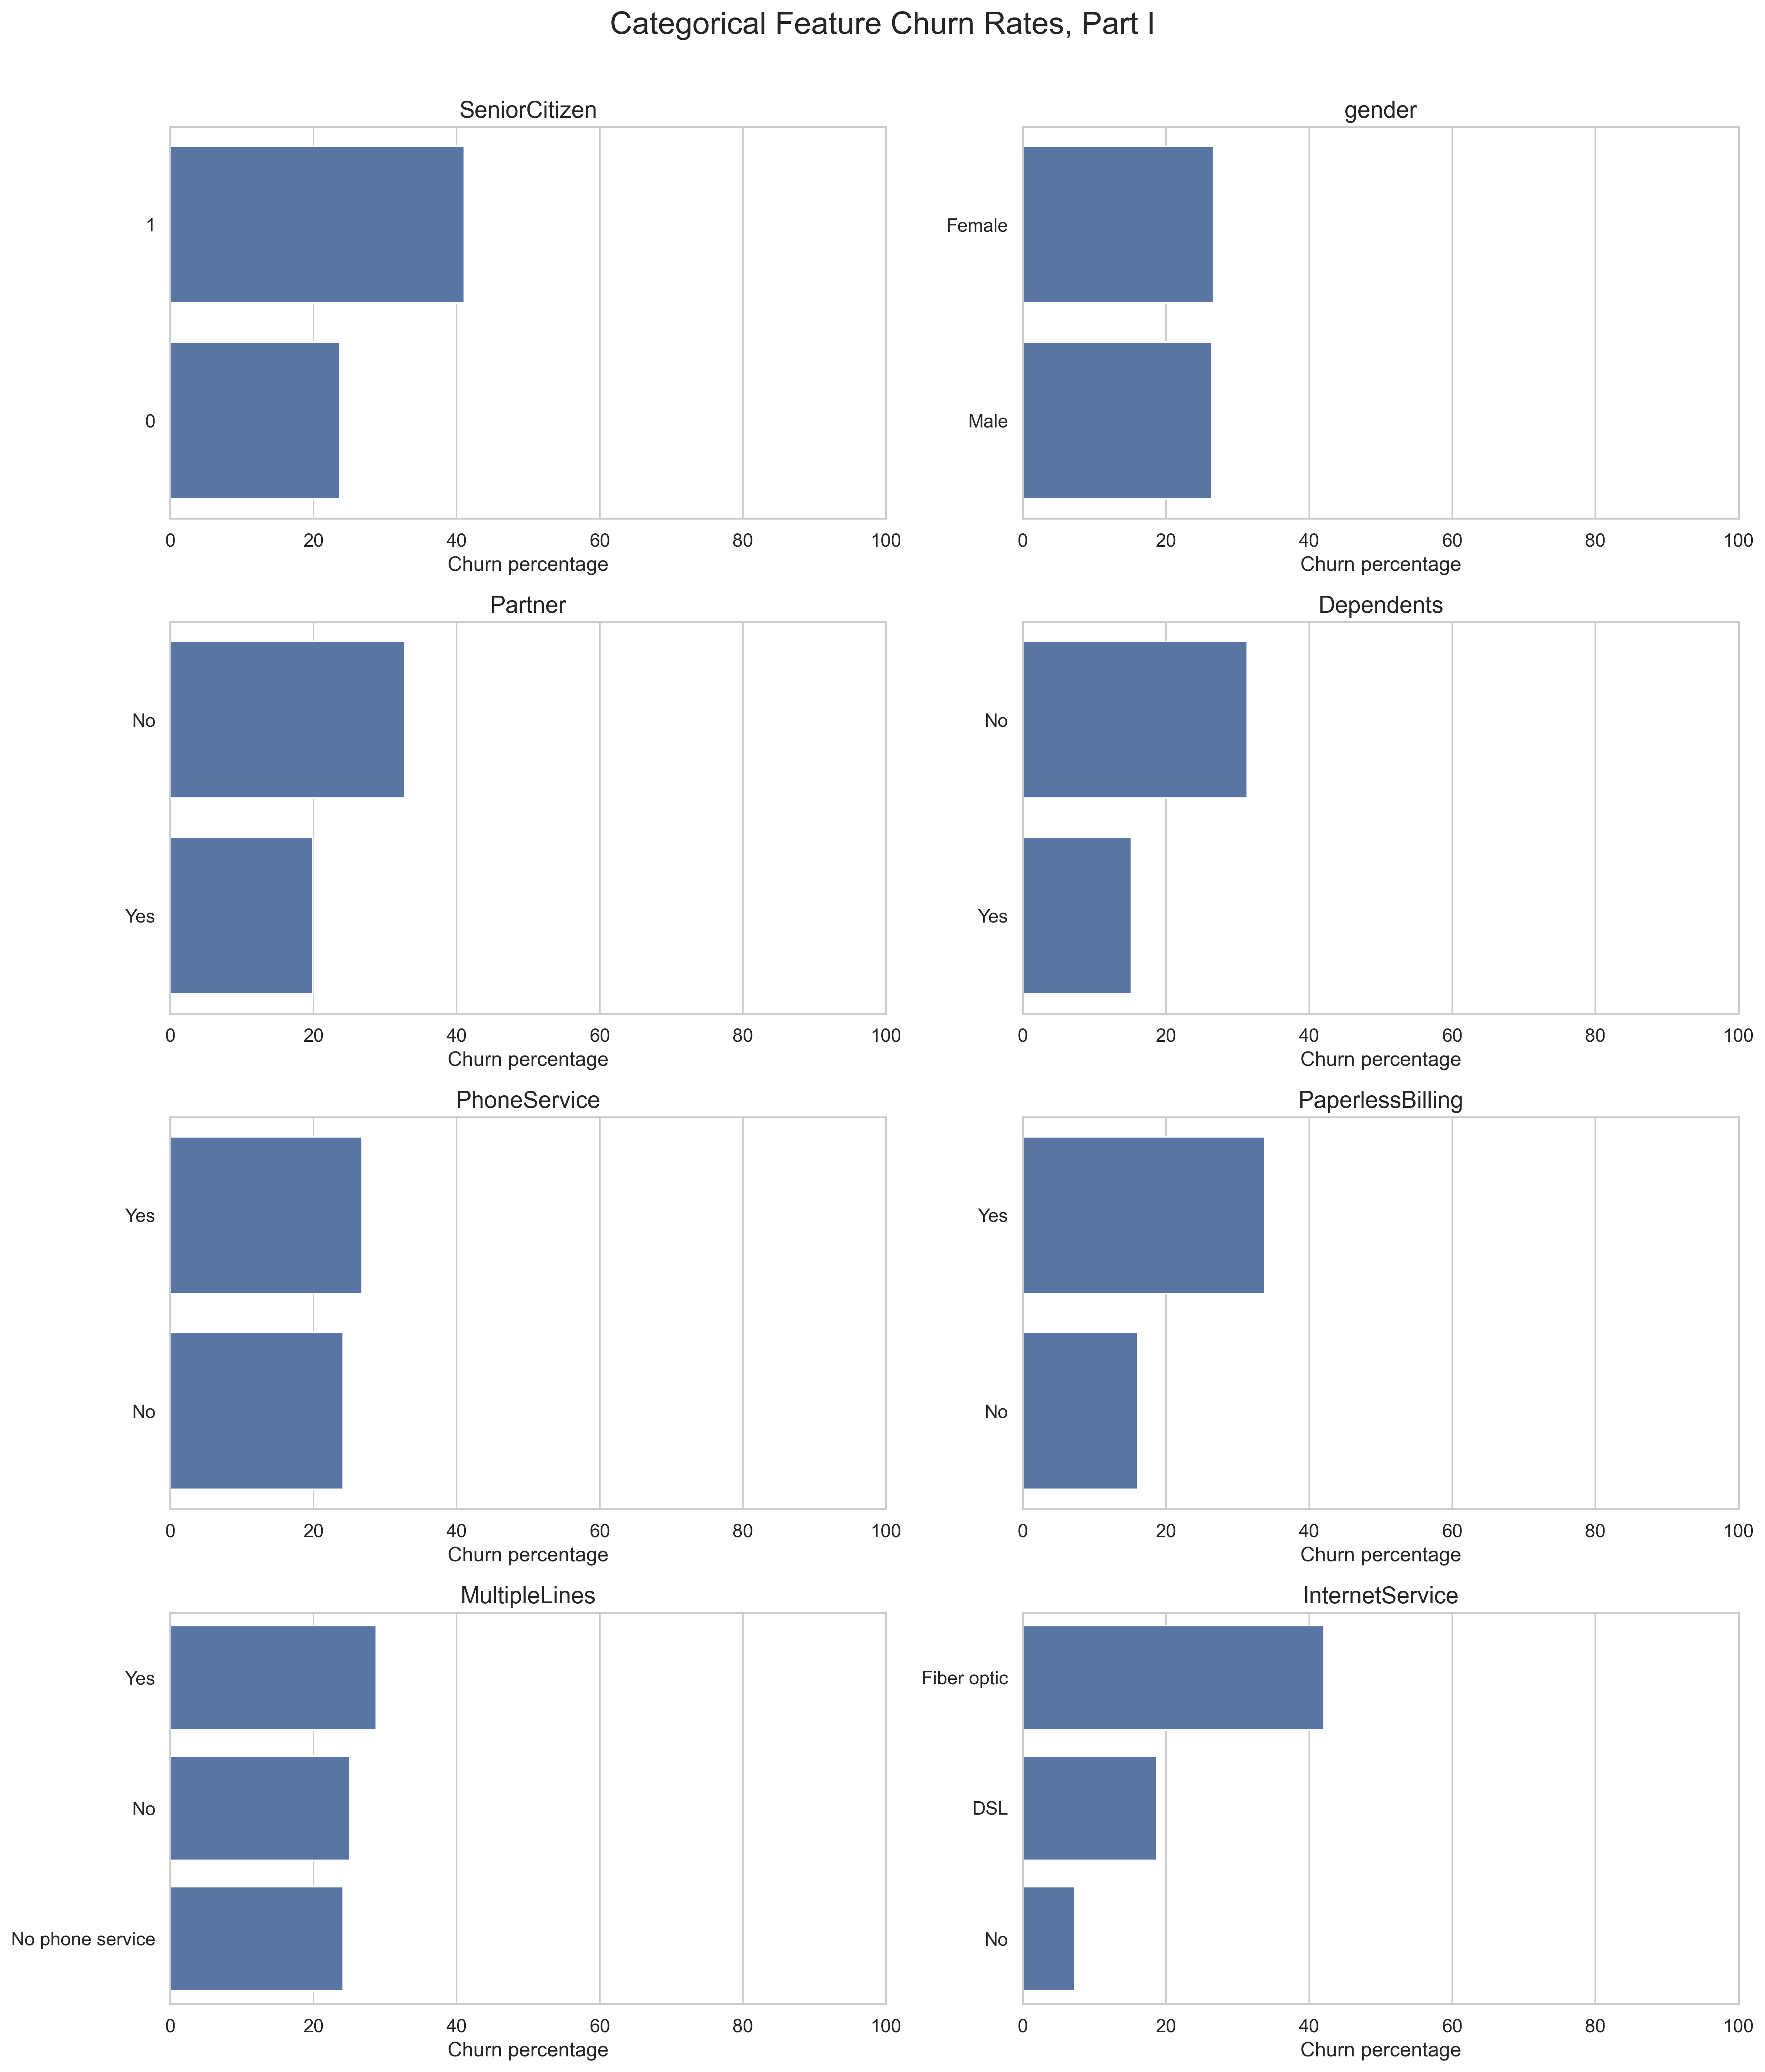
\includegraphics[width=\textwidth]{../figures/training_categorical_feature_churn_rates_part_1.png}
\caption{Categorical feature churn rates, Part I}
\label{fig:training-categorical-churn-rates-part-1}
\end{figure}

\begin{figure}[H]
\centering
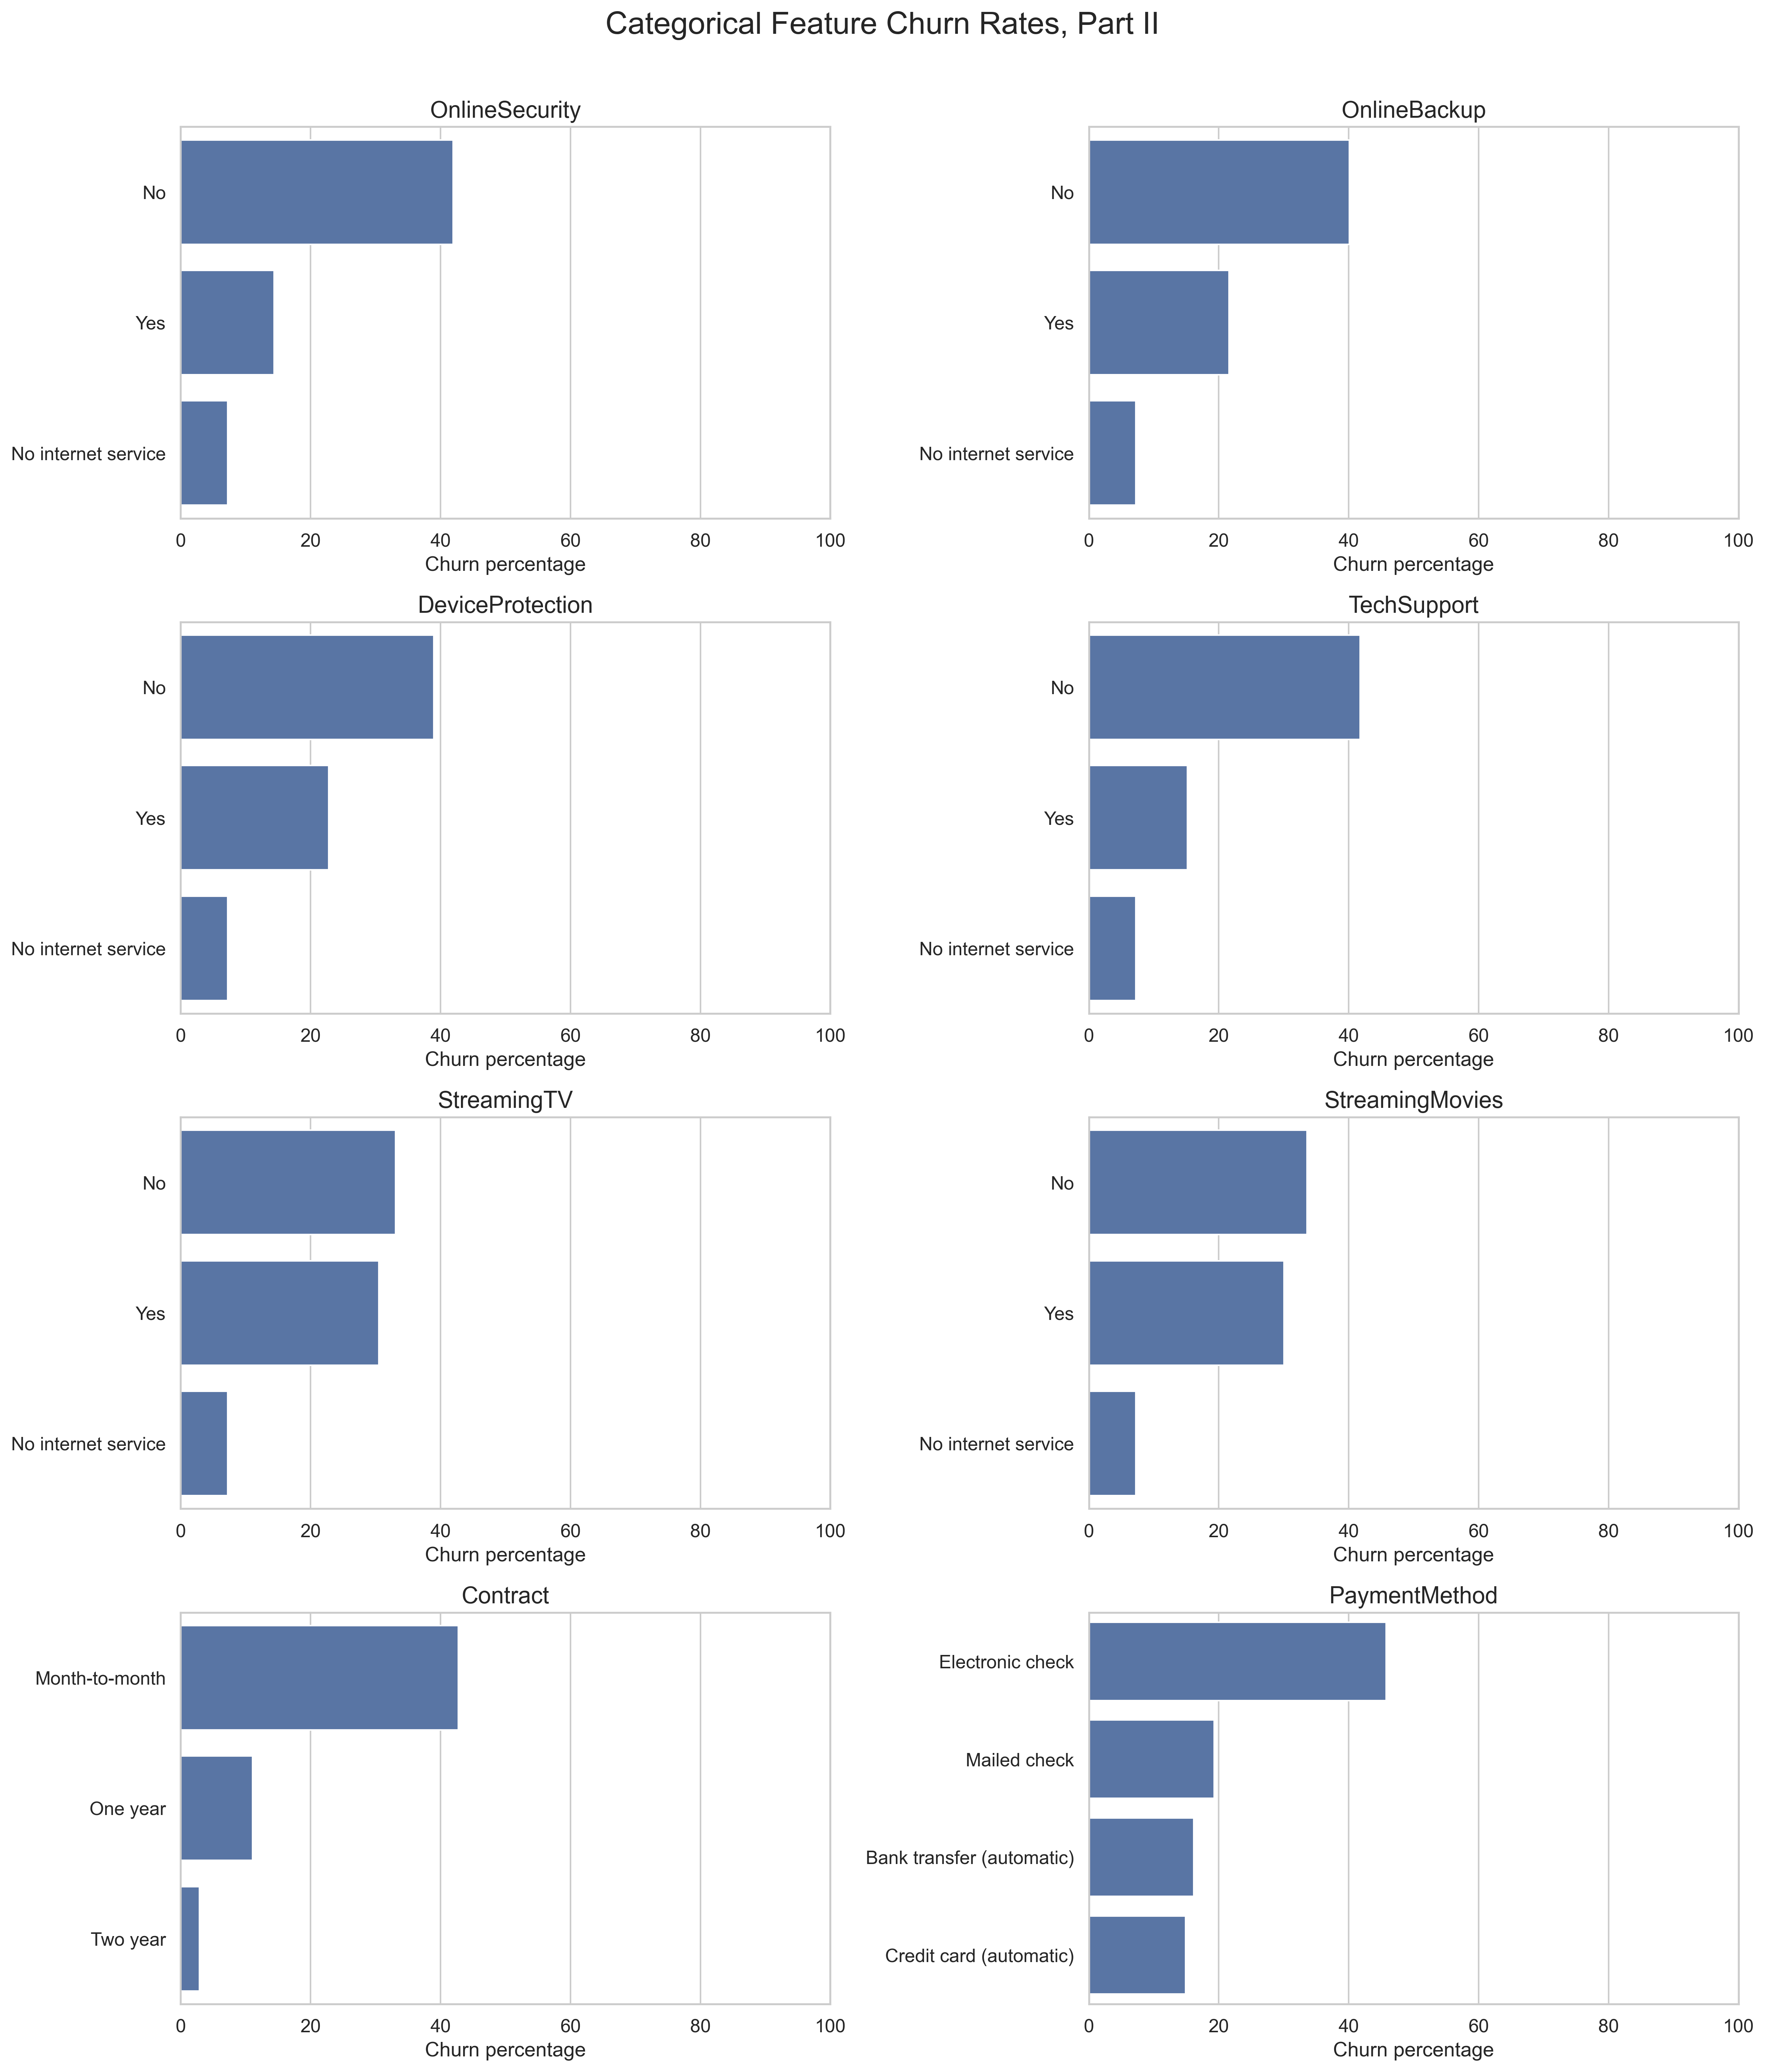
\includegraphics[width=\textwidth]{../figures/training_categorical_feature_churn_rates_part_2.png}
\caption{Categorical feature churn rates, Part II}
\label{fig:training-categorical-churn-rates-part-2}
\end{figure}

The categorical churn-rate plots reveal several large training-set differences. Contract type is one of the strongest categorical patterns: month-to-month customers have a churn rate of 42.75\%, compared with 11.08\% for one-year contracts and 2.87\% for two-year contracts. Internet service type also differs strongly: fiber optic customers have a churn rate of 42.09\%, compared with 18.69\% for DSL and 7.25\% for customers with no internet service.

Payment method is also informative. Customers using electronic check have a churn rate of 45.74\%, higher than mailed check at 19.28\%, bank transfer at 16.16\%, and credit card at 14.92\%. Customers without online security or tech support also show much higher churn rates than customers with those services.

Some variables show weak marginal separation. For example, churn rates for \texttt{gender} are almost identical, and \texttt{PhoneService} shows only a small difference. This does not mean these variables must be removed, because they may still contribute through interactions or in combination with other features. It does suggest that their standalone marginal relationship with churn is weak.

\subsection{Selected categorical churn-rate table}

Table \ref{tab:selected-categorical-churn-rates} reports selected categorical levels that are especially relevant for interpretation and later baseline design.

\begin{table}[H]
\centering
\caption{Selected categorical churn rates}
\label{tab:selected-categorical-churn-rates}
\begin{tabular}{llrrr}
\toprule
Feature & Level & Count & Training \% & Churn \% \\
\midrule
\texttt{Contract} & Month-to-month & 3102 & 55.06 & 42.75 \\
\texttt{Contract} & One year & 1173 & 20.82 & 11.08 \\
\texttt{Contract} & Two year & 1359 & 24.12 & 2.87 \\
\texttt{InternetService} & Fiber optic & 2483 & 44.07 & 42.09 \\
\texttt{InternetService} & DSL & 1937 & 34.38 & 18.69 \\
\texttt{InternetService} & No & 1214 & 21.55 & 7.25 \\
\texttt{PaymentMethod} & Electronic check & 1891 & 33.56 & 45.74 \\
\texttt{PaperlessBilling} & Yes & 3331 & 59.12 & 33.80 \\
\texttt{PaperlessBilling} & No & 2303 & 40.88 & 16.02 \\
\texttt{SeniorCitizen} & 1 & 920 & 16.33 & 41.09 \\
\texttt{SeniorCitizen} & 0 & 4714 & 83.67 & 23.70 \\
\bottomrule
\end{tabular}
\end{table}

These are associations in the training data, not causal effects. They are useful for understanding the dataset, designing simple baselines, and interpreting later models.

\subsection{Summary}

The EDA suggests that the dataset contains meaningful predictive structure. Numerically, churn is most clearly associated with lower tenure and somewhat higher monthly charges. \texttt{TotalCharges} is lower among churners, but this is closely related to the shorter tenure of churned customers.

Categorically, the strongest visible churn-rate differences occur for contract type, internet service type, payment method, online security, tech support, paperless billing, and senior-citizen status. These patterns motivate the next stage: building preprocessing pipelines and baseline classifiers using only the training set.
